\section{Analytical quantities}
\label{sec:analytical}

To understand the dynamical properties of the BDC process, there are a handful
of quantities on which the analysis focuses. We introduce each in turn --- the
non-catastrophe probability, the non-fixation probability, the process mean,
and the expected released count --- stating the closed forms first and deriving
them in Section~\ref{sec:derivations}. Throughout, the process starts from a
single replicative unit, $\xx_0=1$, unless stated otherwise.

\subsection{$I(t)$, the non-catastrophe probability}

\vspace{3pt}
{\Large$$ I(t) = \pr{\xt \neq H\;|\; \xx_0 = 1}$$}

\noindent
Given that the rupture state $H$ is accessible from every non-zero state of the
Markov process, eventual catastrophe is inevitable provided the process does not
first fixate by depletion to $0$. Either death or catastrophe is therefore sure
to happen at late time, and $I(t)$ is the probability that the process has not
experienced catastrophe prior to time $t$.

\begin{theorem}
\label{thm:I}
The non-catastrophe probability is
\begin{equation}
\label{eq:Iclosedform}
I(t) = \frac{aB + bA\,w}{B + A\,w},
\end{equation}
where $w=\ee^{\theta t}$ with $\theta=\lambda(a-b)$, and
\begin{equation*}
a = \eta+\sqrt{\eta^2-\frac{\mu}{\lambda}}, \qquad
b = \eta-\sqrt{\eta^2-\frac{\mu}{\lambda}}, \qquad
\eta = \frac{\lambda + \mu + \delta}{2\lambda},
\end{equation*}
are the two roots, $b<1<a$, of $\lambda x^2-(\lambda+\mu+\delta)x+\mu=0$, while
$A=a-1$ and $B=1-b$.
\end{theorem}

The constants $a$ and $b$ carry the probabilistic content of the formula.
When $\mu>0$, death of the process is possible, and $I(t)$ tends down to the
positive constant value $b$, the likelihood of eventual process death:
$$\lim_{t\to \infty}I(t) = \lim_{t\to\infty}\frac{aB + bAw}{B + Aw} = \frac{bA}{A} = b.$$
When $\mu=0$, death is impossible and $b=0$: catastrophe strikes every
realisation eventually, and $I(t)$ decays to $0$.

\begin{figure}[H]
\centering
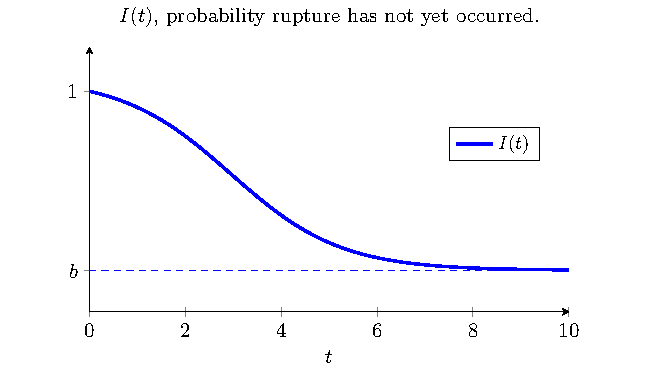
\includegraphics[width = 0.65\textwidth]{figures/I_of_t_1.pdf}
\caption{$I(t)$ plotted against time. It converges to $b$, the probability that the process dies out internally before rupture. $\lambda=1$, $\mu=0.2$, $\delta=0.05$.}
\label{fig:I_of_t_1}
\end{figure}

\subsection{$\Ifix(t)$, the non-fixation probability}

\vspace{3pt}
{\Large$$ \Ifix(t) = \pr{\xt \notin \{0, H \}\;|\; \xx_0 = 1}$$}

\noindent
We can also consider the probability that at time $t$ the process has neither
died out nor experienced catastrophe --- that it remains ``productive''. This is
the non-fixation probability
$$\Ifix(t) = \pr{\xt \notin \{0, H \}\;|\;\xx_0 = 1},$$
which declines asymptotically to $0$, signifying the eventual certainty of
fixation one way or the other. Writing $D(t)=p_0(t)$ for the probability that
the process has died out internally by time $t$, we have, since the absorbing
states $0$ and $H$ exhaust the ways of leaving the productive states,
$$\Ifix(t) = I(t) - D(t).$$
That decomposition pays off immediately: both $I$ and $D$ have closed forms
(Theorems~\ref{thm:I} and~\ref{thm:D}), and their difference simplifies.

\begin{theorem}
\label{thm:D}
The internal-extinction probability is
\begin{equation}
\label{eq:Dclosedform}
D(t) = p_0(t) = \frac{ab(w-1)}{aw-b},
\end{equation}
and the non-fixation probability is
\begin{equation}
\label{eq:Ifixclosedform}
\Ifix(t) = I(t)-D(t) = \frac{(a-b)^2\,w}{(B+Aw)(aw-b)}.
\end{equation}
\end{theorem}

The limits of \eqref{eq:Ifixclosedform} behave as the definition demands:
$\Ifix(0)=1$ (the process begins productive), $\Ifix(\infty)=0$ (fixation is
certain), and the initial slope is $\Ifix'(0)=-(\mu+\delta)$: at the first
instant, a productive realisation is lost either to death at rate $\mu$ or to
catastrophe at rate $\delta$. Notice also the collapse when $\mu=0$: then
$b=0$ and $D(t)=0$ at every $t$, so $\Ifix=I$, and the two quantities of this
section and the last coincide. When $\mu>0$ they are genuinely distinct, and
keeping them apart is what allows the quasi-stationary analysis of
Chapter~4a to condition on continued productivity rather than mere survival of
rupture. \Figref{fig:I_of_t_2} shows $\Ifix(t)$ for the same parameters as
\Figref{fig:I_of_t_1}.

\begin{figure}[H]
\centering
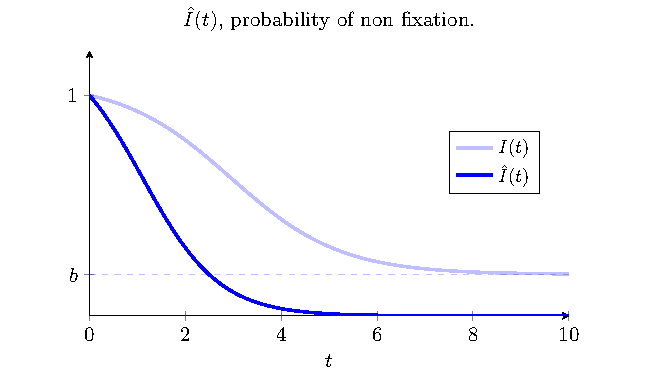
\includegraphics[width = 0.65\textwidth]{figures/I_of_t_2.pdf}
\caption{$\Ifix(t)$ plotted against time. $\lambda=1$, $\mu=0.2$, $\delta=0.05$.}
\label{fig:I_of_t_2}
\end{figure}

\figureflag{F3.3}{Fixation functions}{%
\textbf{Purpose:} show the three survival-type functions $I(t)$, $D(t)$ and
$\Ifix(t)$ together, making visible that $I$ and $D$ share the limit $b$ while
$\Ifix=I-D$ decays to $0$ --- the decomposition on which the quasi-stationary
analysis of Chapter~4a rests. \textbf{Type:} Python analytic plot.
\textbf{Content:} three curves on $t\in[0,15]$ for
$(\lambda,\mu,\delta)=(1,0.2,0.05)$, evaluated from the closed forms of
Theorems~\ref{thm:I} and~\ref{thm:D}:
$I(t)=(aB+bAw)/(B+Aw)$, $D(t)=ab(w-1)/(aw-b)$,
$\Ifix(t)=(a-b)^2w/((B+Aw)(aw-b))$, with $w=e^{\theta t}$,
$\theta=\lambda(a-b)$; horizontal dashed asymptotes at $b$ (for $I$ and $D$)
and at $0$ (for $\Ifix$); annotate the initial slope
$\Ifix'(0)=-(\mu+\delta)=-0.25$ near $t=0$. \textbf{Axes:} $t$ (horizontal,
0--15), probability (vertical, 0--1); legend entries $I(t)$, $D(t)$,
$\Ifix(t)$. \textbf{Style:} unified Python style --- default matplotlib with
\texttt{tab:} colours, grid alpha 0.25, \texttt{tight\_layout}, PDF output,
fonts matching the chapter. \textbf{Data source:} analytic formulas above; no
simulation. \textbf{Placement:} \Secref{sec:analytical}, after the discussion
of $\Ifix(t)$ and before the subsection on $J(t)$.}

\subsection{Multiple founders}

Suppose the process begins with $k$ initial particles, $\xx_0 = k$. Each
replicative unit gives rise to its own family of descendants, all behaving
independently of one another, so probabilities for the whole population factor
into per-family probabilities (the branching property). The likelihood that any
one of those $k$ families will \textit{not} have led to catastrophe by time $t$
is $I(t)$; hence the probability that none of the $k$ families has caused the
mass emigration is
$$I_k(t) = \pr{\xt \neq H\;|\; \xx_0 = k} = \lrbs{I(t)}^k.$$
Likewise, internal extinction of the whole population requires every family to
die out, giving $D_k(t)=D(t)^k$, and for non-fixation more generally,
$$\Ifix[,{k}](t) = \pr{\xt \notin \{0, H \}\;|\; \xx_0 = k} = I(t)^k - D(t)^k.$$
The tempting simplification $\Ifix[,{k}]=\Ifix^k$ is false when $\mu>0$:
non-fixation of the whole population fails as soon as \textit{any one} family
fixates, whether by death or by rupture, and the two routes must be separated
exactly as above. (When $\mu=0$, $D=0$ and the two expressions do coincide.)
The multi-founder quantities return in Chapter~4a, where they are derived from
the probability generating functions and used to describe cells infected by
several particles at once.

\subsection{$J(t)$, the replicative unit mean}

\vspace{3pt}
{\Large$$J(t) = \mean{\xt\;|\;\xx_0 = 1}$$}

\noindent
A given realisation of the process will rise and fall stochastically in steps
for some time before ending up stuck either at $0$ or, after catastrophe, at
$H$. Following each of these fixation outcomes, the contribution of $\xt$ to
the mean $J(t)$ is $0$. So, supposing we observe 100 realisations, if at time
$t=20$ all of them have either died or undergone catastrophe, their sample mean
would be $0$ ($J_{\text{sample}}(20) = 0$). From the initial condition
$\xx_0 = 1$, the process mean rises while realisations tend to increase, then
falls as the likelihood of fixation grows asymptotically certain.

\begin{figure}[H]
\centering
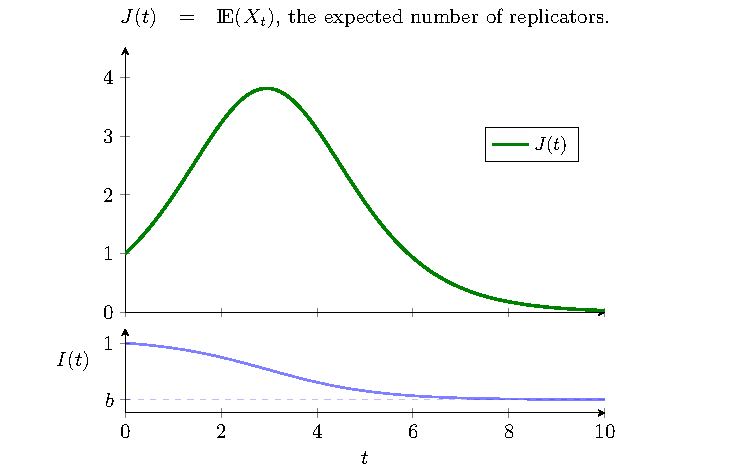
\includegraphics[width = 0.7\textwidth]{figures/J_of_t_1.pdf}
\caption{$J(t)$ plotted against time. $\lambda=1$, $\mu=0.2$, $\delta=0.05$.}
\label{fig:J_of_t_1}
\end{figure}

\begin{theorem}
\label{thm:J}
The expected process state is
\begin{equation}
\label{eq:Jclosedform}
J(t) = \frac{(a-b)^2\,w}{(B+Aw)^2} = -\frac{\lambda}{\delta}(I-a)(I-b),
\end{equation}
obtained by differentiating $I(t)$ and multiplying by $-\delta^{-1}$, using the
relation $I'=-\delta J$ established in Section~\ref{sec:derivations}.
\end{theorem}

\noindent
The second form of \eqref{eq:Jclosedform}, written purely in terms of $I$, is
the one that will do most of the work later: it expresses the mean load as a
function of the non-catastrophe probability alone.

\figureflag{F3.4}{Conditional mean convergence}{%
\textbf{Purpose:} show the quasi-stationary level of the process --- the
conditional mean $J/\Ifix$ tending to a constant while the unconditional mean
$J$ dies away --- before the quasi-stationary distribution is formally defined
in Chapter~4a. \textbf{Type:} Python analytic plot, two panels.
\textbf{Content:} panel (a): $\mu=0$, $(\lambda,\delta)=(1,0.1)$, curves of
$J(t)/I(t)$ and of $V(t)$ on $t\in[0,15]$, both tending to
$1+\lambda/\delta=11$; horizontal dashed asymptote at $11$. Panel (b):
$\mu>0$, $(\lambda,\mu,\delta)=(1,0.2,0.05)$, curves of $J(t)/\Ifix(t)$
tending to $a/(a-1)$ and of $J(t)/I(t)$ tending to $0$, on $t\in[0,15]$, with
dashed asymptotes at $a/(a-1)$ and $0$. Use the closed forms of
Theorems~\ref{thm:I} and~\ref{thm:J} and $V(t)=(1-I)[1+\frac{\lambda}{\delta}(1-I)]$.
\textbf{Axes:} $t$ (horizontal), conditional mean (vertical); legend entries
$J/I$ or $J/\Ifix$ as appropriate. \textbf{Style:} unified Python style ---
default matplotlib with \texttt{tab:} colours, grid alpha 0.25,
\texttt{tight\_layout}, PDF output, fonts matching the chapter.
\textbf{Data source:} analytic formulas; no simulation. \textbf{Placement:}
\Secref{sec:analytical}, directly after \Figref{fig:J_of_t_1} or the theorem
for $J(t)$.}

\subsection{$V(t)$, the expected number of released units}

\vspace{3pt}
{\Large$$V(t) = \mean{\wt\;|\; \xx_0 = 1}$$}

\noindent
Over time, the process will either decline to $0$, or transition to the
catastrophe state $H$, in which case $\wt$ is set at the final value of $\xt$
before rupture. $V(t)$, the expected post-rupture count, incorporates all
situations, whether $\wt$ is zero or not.

\begin{theorem}
\label{thm:V}
The expected released count is
\begin{equation}
\label{eq:Vclosedform}
V(t) = (1-I)\Bigl[1+\frac{\lambda}{\delta}(1-I)\Bigr]
= \frac{(\lambda - \mu)}{\delta}\big[1-I(t)\big] -J(t)+1,
\end{equation}
and its late-time value is
\begin{equation}
\label{eq:Vinf}
V_{\infty} = \lim_{t\to\infty}V(t) = \frac{aB}{A} =
\frac{\lambda-\mu}{\delta}(1-b)+1,
\end{equation}
as $I\to b$ and $J\to0$. When $\mu=0$, this reduces to
$V_{\infty} = 1+\lambda/\delta$.
\end{theorem}

\begin{figure}[H]
\centering
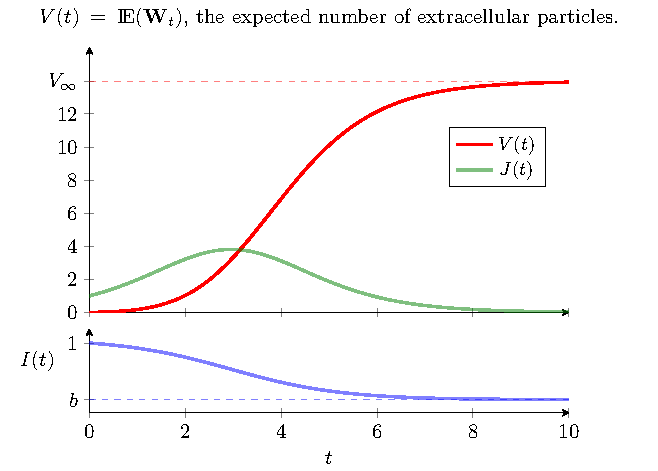
\includegraphics[width = 0.7\textwidth]{figures/V_of_t_1.pdf}
\caption{$V(t)$ plotted against time. $\lambda=1$, $\mu=0.2$, $\delta=0.05$.}
\label{fig:V_of_t_1}
\end{figure}

For the case where death is included ($\mu>0$), $V_{\infty}$ takes into
account eventualities in which the process did not attain catastrophe --- the
dead realisations contribute nothing to the release. We may extract the mean
burst size proper by conditioning on the cases which did experience rupture,
effectively discounting the dead realisations. This is done by dividing $V(t)$
by the likelihood of process catastrophe, $1-I(t)$, following the basic logic
$$\mean{\wt} = \cancelto{0}{\mean{\wt \,|\, \text{no rupture}}\, I(t) }  + \mean{\wt \,|\, \text{rupture}}\, (1 - I(t)),$$
so that
$$\mean{\wt \,|\, \text{rupture}}  =  \frac{\mean{\wt}}{1 - I(t)}.$$
The ratio $V(t)/[1 - I(t)]$ represents the expected burst size given that
catastrophe has taken place by time $t$. The overall mean burst size,
incorporating all realisations which experience rupture regardless of when, is
the late-time value of this ratio:

\begin{corollary}
\label{cor:burstmean}
The mean burst size, conditional on bursting eventually, is
\begin{equation}
\label{eq:burstmean}
\mean{\Kb \,|\,\text{burst}} = \lim_{t\to \infty} \frac{V(t)}{1 - I(t)}
= \frac{V_{\infty}}{1 - b}
= \frac{\lambda-\mu}{\delta} + \frac{1}{1-b}
= \frac{a}{a-1},
\end{equation}
recalling that $b$ is the probability of ultimate process death. Notice the
alignment $\mean{\Kb\,|\,\text{burst}} = V_\infty$ when $\mu=0$, since then
every realisation bursts.
\end{corollary}

The full distribution of the burst size $\Kb$, not only its mean, is derived in
Chapter~4a; a preview of its geometric form appears in
Section~\ref{sec:whatnext}.
